% Options for packages loaded elsewhere
\PassOptionsToPackage{unicode}{hyperref}
\PassOptionsToPackage{hyphens}{url}
\PassOptionsToPackage{dvipsnames,svgnames,x11names}{xcolor}
%
\documentclass[
  letterpaper,
  DIV=11,
  numbers=noendperiod,
  oneside]{scrartcl}

\usepackage{amsmath,amssymb}
\usepackage{iftex}
\ifPDFTeX
  \usepackage[T1]{fontenc}
  \usepackage[utf8]{inputenc}
  \usepackage{textcomp} % provide euro and other symbols
\else % if luatex or xetex
  \usepackage{unicode-math}
  \defaultfontfeatures{Scale=MatchLowercase}
  \defaultfontfeatures[\rmfamily]{Ligatures=TeX,Scale=1}
\fi
\usepackage{lmodern}
\ifPDFTeX\else  
    % xetex/luatex font selection
\fi
% Use upquote if available, for straight quotes in verbatim environments
\IfFileExists{upquote.sty}{\usepackage{upquote}}{}
\IfFileExists{microtype.sty}{% use microtype if available
  \usepackage[]{microtype}
  \UseMicrotypeSet[protrusion]{basicmath} % disable protrusion for tt fonts
}{}
\makeatletter
\@ifundefined{KOMAClassName}{% if non-KOMA class
  \IfFileExists{parskip.sty}{%
    \usepackage{parskip}
  }{% else
    \setlength{\parindent}{0pt}
    \setlength{\parskip}{6pt plus 2pt minus 1pt}}
}{% if KOMA class
  \KOMAoptions{parskip=half}}
\makeatother
\usepackage{xcolor}
\usepackage[left=1in,marginparwidth=2.0666666666667in,textwidth=4.1333333333333in,marginparsep=0.3in]{geometry}
\setlength{\emergencystretch}{3em} % prevent overfull lines
\setcounter{secnumdepth}{5}
% Make \paragraph and \subparagraph free-standing
\makeatletter
\ifx\paragraph\undefined\else
  \let\oldparagraph\paragraph
  \renewcommand{\paragraph}{
    \@ifstar
      \xxxParagraphStar
      \xxxParagraphNoStar
  }
  \newcommand{\xxxParagraphStar}[1]{\oldparagraph*{#1}\mbox{}}
  \newcommand{\xxxParagraphNoStar}[1]{\oldparagraph{#1}\mbox{}}
\fi
\ifx\subparagraph\undefined\else
  \let\oldsubparagraph\subparagraph
  \renewcommand{\subparagraph}{
    \@ifstar
      \xxxSubParagraphStar
      \xxxSubParagraphNoStar
  }
  \newcommand{\xxxSubParagraphStar}[1]{\oldsubparagraph*{#1}\mbox{}}
  \newcommand{\xxxSubParagraphNoStar}[1]{\oldsubparagraph{#1}\mbox{}}
\fi
\makeatother


\providecommand{\tightlist}{%
  \setlength{\itemsep}{0pt}\setlength{\parskip}{0pt}}\usepackage{longtable,booktabs,array}
\usepackage{calc} % for calculating minipage widths
% Correct order of tables after \paragraph or \subparagraph
\usepackage{etoolbox}
\makeatletter
\patchcmd\longtable{\par}{\if@noskipsec\mbox{}\fi\par}{}{}
\makeatother
% Allow footnotes in longtable head/foot
\IfFileExists{footnotehyper.sty}{\usepackage{footnotehyper}}{\usepackage{footnote}}
\makesavenoteenv{longtable}
\usepackage{graphicx}
\makeatletter
\newsavebox\pandoc@box
\newcommand*\pandocbounded[1]{% scales image to fit in text height/width
  \sbox\pandoc@box{#1}%
  \Gscale@div\@tempa{\textheight}{\dimexpr\ht\pandoc@box+\dp\pandoc@box\relax}%
  \Gscale@div\@tempb{\linewidth}{\wd\pandoc@box}%
  \ifdim\@tempb\p@<\@tempa\p@\let\@tempa\@tempb\fi% select the smaller of both
  \ifdim\@tempa\p@<\p@\scalebox{\@tempa}{\usebox\pandoc@box}%
  \else\usebox{\pandoc@box}%
  \fi%
}
% Set default figure placement to htbp
\def\fps@figure{htbp}
\makeatother

% load packages
\usepackage{geometry}
\usepackage{xcolor}
\usepackage{eso-pic}
\usepackage{fancyhdr}
\usepackage{sectsty}
\usepackage{fontspec}
\usepackage{titlesec}

%% Set page size with a wider right margin
\geometry{a4paper, total={170mm,257mm}, left=20mm, top=20mm, bottom=20mm, right=50mm}

%% Let's define some colours
\definecolor{uniblue}{HTML}{003865}
\definecolor{burgundy}{HTML}{7D2239}
\definecolor{cobalt}{HTML}{005C8A}
\definecolor{lavender}{HTML}{5B4D94}
\definecolor{leaf}{HTML}{006630}
\definecolor{moss}{HTML}{385A4F}
\definecolor{pillarbox}{HTML}{B30C00}
\definecolor{rust}{HTML}{9A3A06}
\definecolor{sandstone}{HTML}{52473B}
\definecolor{skyblue}{HTML}{005398}
\definecolor{slate}{HTML}{4F5961}
\definecolor{thistle}{HTML}{951272}

%\definecolor{light}{HTML}{E6E6FA} % original from template - redefined below as uni blue at 10 percent:
\colorlet{light}{uniblue!10}
%\definecolor{highlight}{HTML}{800080} % original from template - redefined below as uni's skyblue:
\colorlet{highlight}{skyblue}
%\definecolor{dark}{HTML}{330033} % original from template - redefined below as uni blue at 100 percent:
\colorlet{dark}{uniblue}

%% Let's add the border on the right hand side 
\AddToShipoutPicture{% 
    \AtPageLowerLeft{% 
        \put(\LenToUnit{\dimexpr\paperwidth-3cm},0){% 
            \color{light}\rule{3cm}{\LenToUnit\paperheight}%
          }%
     }%
     % logo
    \AtPageLowerLeft{% start the bar at the bottom right of the page
        \put(\LenToUnit{\dimexpr\paperwidth-2.25cm},27.2cm){% move it to the top right
            \color{light}
\includegraphics[width=2.25cm]{_extensions/nrennie/PrettyPDF/uni_logo_boxed.jpg}
          }%
     }%
}

%% Style the page number
\fancypagestyle{mystyle}{
  \fancyhf{}
  \renewcommand\headrulewidth{0pt}
  \fancyfoot[R]{\thepage}
  \fancyfootoffset{3.5cm}
}
\setlength{\footskip}{20pt}

%% style the chapter/section fonts
\chapterfont{\color{uniblue}\fontsize{20}{16.8}\selectfont}
\sectionfont{\color{uniblue}\fontsize{20}{16.8}\selectfont}
\subsectionfont{\color{skyblue}\fontsize{14}{16.8}\selectfont}
\titleformat{\subsection}
  {\color{uniblue!90}\sffamily\Large\bfseries}{\thesubsection}{1em}{}[{\titlerule[0.8pt]}]
\subsubsectionfont{\color{cobalt}}

\renewcommand\thesection{\color{slate}\arabic{section}}
  
% left align title
\makeatletter
\renewcommand{\maketitle}{\bgroup\setlength{\parindent}{0pt}
\begin{flushleft}
  {\color{uniblue}\sffamily\huge\textbf{\@title}} \vspace{0.3cm} \newline
  {\Large {\@subtitle}} \newline
  \@author
\end{flushleft}\egroup
}
\makeatother

%%% Use some custom fonts
\setsansfont{Ubuntu}[
    Path=_extensions/nrennie/PrettyPDF/Ubuntu/,
    Scale=0.9,
    Extension = .ttf,
    UprightFont=*-Regular,
    BoldFont=*-Bold,
    ItalicFont=*-Italic,
    ]

\setmainfont{Ubuntu}[
    Path=_extensions/nrennie/PrettyPDF/Ubuntu/,
    Scale=0.9,
    Extension = .ttf,
    UprightFont=*-Regular,
    BoldFont=*-Bold,
    ItalicFont=*-Italic,
    ]
\KOMAoption{captions}{tableheading}
\makeatletter
\@ifpackageloaded{tcolorbox}{}{\usepackage[skins,breakable]{tcolorbox}}
\@ifpackageloaded{fontawesome5}{}{\usepackage{fontawesome5}}
\definecolor{quarto-callout-color}{HTML}{909090}
\definecolor{quarto-callout-note-color}{HTML}{0758E5}
\definecolor{quarto-callout-important-color}{HTML}{CC1914}
\definecolor{quarto-callout-warning-color}{HTML}{EB9113}
\definecolor{quarto-callout-tip-color}{HTML}{00A047}
\definecolor{quarto-callout-caution-color}{HTML}{FC5300}
\definecolor{quarto-callout-color-frame}{HTML}{acacac}
\definecolor{quarto-callout-note-color-frame}{HTML}{4582ec}
\definecolor{quarto-callout-important-color-frame}{HTML}{d9534f}
\definecolor{quarto-callout-warning-color-frame}{HTML}{f0ad4e}
\definecolor{quarto-callout-tip-color-frame}{HTML}{02b875}
\definecolor{quarto-callout-caution-color-frame}{HTML}{fd7e14}
\makeatother
\makeatletter
\@ifpackageloaded{caption}{}{\usepackage{caption}}
\AtBeginDocument{%
\ifdefined\contentsname
  \renewcommand*\contentsname{Table of contents}
\else
  \newcommand\contentsname{Table of contents}
\fi
\ifdefined\listfigurename
  \renewcommand*\listfigurename{List of Figures}
\else
  \newcommand\listfigurename{List of Figures}
\fi
\ifdefined\listtablename
  \renewcommand*\listtablename{List of Tables}
\else
  \newcommand\listtablename{List of Tables}
\fi
\ifdefined\figurename
  \renewcommand*\figurename{Figure}
\else
  \newcommand\figurename{Figure}
\fi
\ifdefined\tablename
  \renewcommand*\tablename{Table}
\else
  \newcommand\tablename{Table}
\fi
}
\@ifpackageloaded{float}{}{\usepackage{float}}
\floatstyle{ruled}
\@ifundefined{c@chapter}{\newfloat{codelisting}{h}{lop}}{\newfloat{codelisting}{h}{lop}[chapter]}
\floatname{codelisting}{Listing}
\newcommand*\listoflistings{\listof{codelisting}{List of Listings}}
\makeatother
\makeatletter
\makeatother
\makeatletter
\@ifpackageloaded{caption}{}{\usepackage{caption}}
\@ifpackageloaded{subcaption}{}{\usepackage{subcaption}}
\makeatother
\makeatletter
\@ifpackageloaded{tcolorbox}{}{\usepackage[skins,breakable]{tcolorbox}}
\makeatother
\makeatletter
\@ifundefined{shadecolor}{\definecolor{shadecolor}{rgb}{.97, .97, .97}}{}
\makeatother
\makeatletter
\@ifundefined{codebgcolor}{\definecolor{codebgcolor}{named}{light}}{}
\makeatother
\makeatletter
\ifdefined\Shaded\renewenvironment{Shaded}{\begin{tcolorbox}[colback={codebgcolor}, sharp corners, breakable, frame hidden, boxrule=0pt, enhanced]}{\end{tcolorbox}}\fi
\makeatother
\makeatletter
\@ifpackageloaded{sidenotes}{}{\usepackage{sidenotes}}
\@ifpackageloaded{marginnote}{}{\usepackage{marginnote}}
\makeatother

\usepackage{bookmark}

\IfFileExists{xurl.sty}{\usepackage{xurl}}{} % add URL line breaks if available
\urlstyle{same} % disable monospaced font for URLs
\hypersetup{
  pdftitle={Tutorial Sheet 2},
  colorlinks=true,
  linkcolor={highlight},
  filecolor={Maroon},
  citecolor={Blue},
  urlcolor={highlight},
  pdfcreator={LaTeX via pandoc}}


\title{Tutorial Sheet 2}
\author{}
\date{}

\begin{document}
\maketitle

\pagestyle{mystyle}


\section{Part A: Seasonal and trend
analysis.}\label{part-a-seasonal-and-trend-analysis.}

\begin{tcolorbox}[enhanced jigsaw, colframe=quarto-callout-note-color-frame, toptitle=1mm, toprule=.15mm, bottomtitle=1mm, titlerule=0mm, coltitle=black, left=2mm, rightrule=.15mm, arc=.35mm, colback=white, title=\textcolor{quarto-callout-note-color}{\faInfo}\hspace{0.5em}{Note}, breakable, opacitybacktitle=0.6, opacityback=0, bottomrule=.15mm, leftrule=.75mm, colbacktitle=quarto-callout-note-color!10!white]

Several of these examples are similar in nature to exam questions, in
that you are asked to comment on statements being made or on analysis
already completed.

\end{tcolorbox}

\begin{tcolorbox}[enhanced jigsaw, colframe=quarto-callout-warning-color-frame, toptitle=1mm, toprule=.15mm, bottomtitle=1mm, titlerule=0mm, coltitle=black, left=2mm, rightrule=.15mm, arc=.35mm, colback=white, title={Task 1}, breakable, opacitybacktitle=0.6, opacityback=0, bottomrule=.15mm, leftrule=.75mm, colbacktitle=quarto-callout-warning-color!10!white]

It is of interest to look at temperature records in Loch Lomond and to
consider what the trend might be in water temperature. The data shown
here are for Cailness in the north basin of the Loch. Comment on the
patterns over time in this record. What other plots might you look at
and how might you model this data to investigate the changes in
temperature over time. There are some missing data values which you
might consider how to impute.

\begin{figure}[H]

{\centering 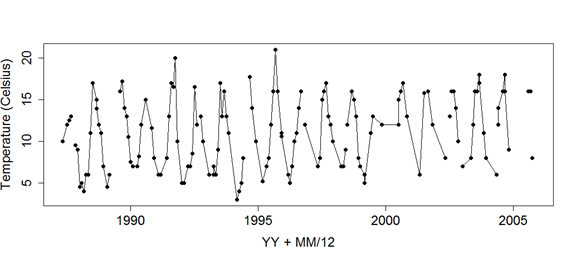
\includegraphics[width=5.53125in,height=\textheight,keepaspectratio]{images/Cailness.png}

}

\caption{Figure 2: Cailness temperature over time}

\end{figure}%

Solution

Temperature records- here the approach since we have approximately
monthly data requires both a trend and seasonality term, since we expect
that temperature will be seasonal. This is a very similar problem to
what we will look at with the Central England temperature record, in the
lab. I would expect to see a time series plot of these data (with time
expressed as year.decimal part of the year), and a seasonality plot,
where each temperature is plotted against position within the year. This
latter plot will for sure show a seasonal cycle and we could easily
imagine fitting some sort of sin/cosine curve to this, hence the idea to
use a harmonic regression. However we also have a problem in that there
is some missing data, and so as a discussion point we could consider how
best to impute these missing values.

Imputation rules (this again would be more typical of an exam style
question): Possible answers here could range from replacement by a
simple average of the values surrounding the missing value, to a more
complex approach which would also use the seasonal signal (e.g.~if the
value was missing in January 2006, you could replace the missing value
by the average of the January 2005 and Jan 2007 values). You could also
use the fitted sine/cosine seasonal curve as a tool for imputation.

You could be asked to look at the original equation for the harmonic
regression (which is non-linear in the params) and show how it can be
linearised (straight from the notes).

\end{tcolorbox}

\begin{tcolorbox}[enhanced jigsaw, colframe=quarto-callout-warning-color-frame, toptitle=1mm, toprule=.15mm, bottomtitle=1mm, titlerule=0mm, coltitle=black, left=2mm, rightrule=.15mm, arc=.35mm, colback=white, title={Task 2}, breakable, opacitybacktitle=0.6, opacityback=0, bottomrule=.15mm, leftrule=.75mm, colbacktitle=quarto-callout-warning-color!10!white]

The following excerpts are taken from the National Snow and Ice Data
Centre (NSIDC) site, concerning arctic sea ice:

\textbf{Statement 3a}

\emph{``Arctic sea ice extent in January 2012 averaged 13.73 million
square kilometers (5.30 million square miles). This is the fourth-lowest
January ice extent in the 1979 to 2012 satellite data record, 1.10
million square kilometers (425,000 square miles) below the 1979 to 2000
average extent. Including the year 2012, the linear rate of decline for
January ice extent over the satellite record is 3.2\% per decade. Based
on the satellite record, before 2005, average January ice extent had
never been lower than 14 million square kilometers (5.41 million square
miles). January ice extent has now fallen below that mark six out of the
last seven years.''}

\textbf{Statement 3b}

\emph{``The growth rate for Arctic sea ice in January was the slowest in
the satellite record. After growing relatively quickly early in January,
ice extent declined briefly in the middle of the month, and then grew
more slowly than normal for the rest of the month. Overall, the Arctic
gained 765,000 square kilometers (295,000 square miles) of ice during
the month. This was 545,000 square kilometers (210,000 square miles)
less than the average ice growth rate for January 1979 to 2000.''}

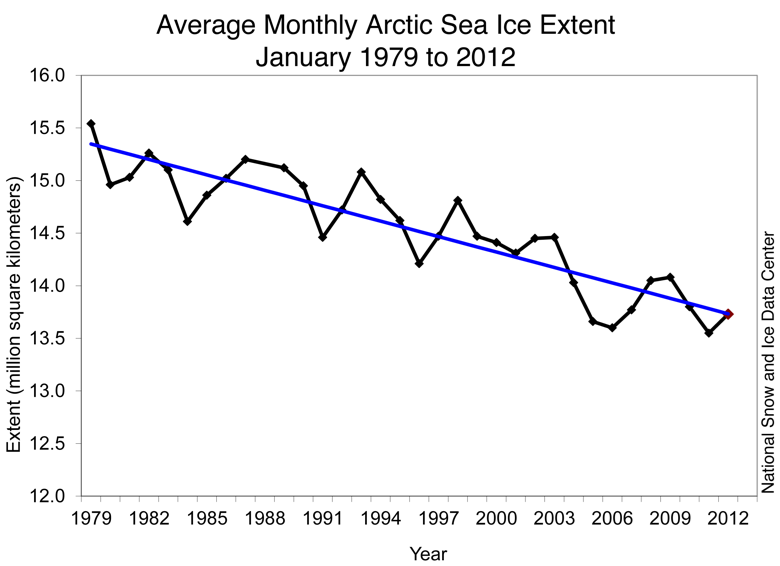
\includegraphics[width=4.64583in,height=\textheight,keepaspectratio]{images/jan_sea_ice_extent.png}
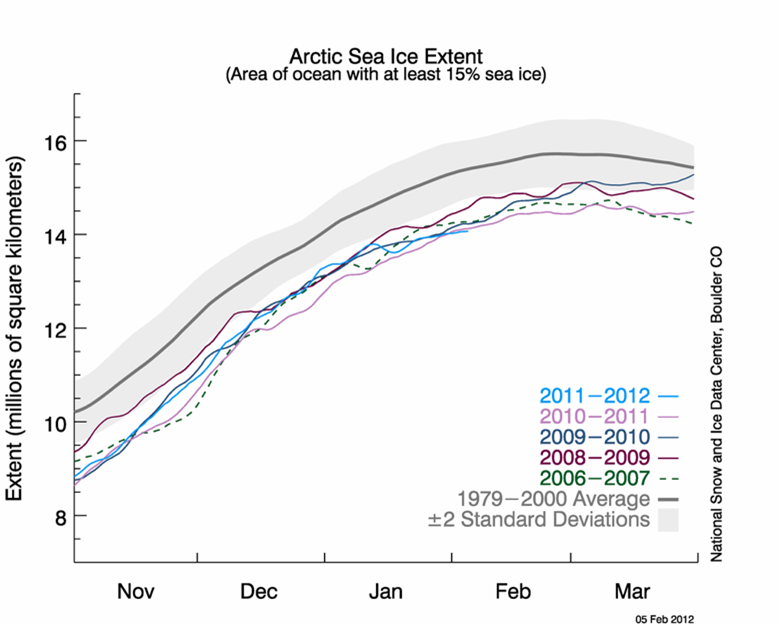
\includegraphics[width=4.64583in,height=\textheight,keepaspectratio]{images/ann_sea_ice_extent.png}

Discuss critically the two statements above concerning the 2012 sea-ice
making reference to Figures 3.1 and 3.2, specifically the decrease per
decade. Comment on the statistical methods and assumption which could be
used to fit the models shown in the Figures. How would you interpret
Figure 3.2 in terms of the comparison of the 5 curves shown to the
1979-2000 average curve?

Solution

Statement 3a, several aspects to comment on, the most straightforward
concerns the linear rate of decline (3.2\% per decade), no uncertainty
mentioned. Fig 3.1, shows the straight line fit and the fluctuations
around the line (why no uncertainty bands?). The second aspect to
comment on really is about the rank information, fourth lowest, and
January ice extent fallen below 14 million km\(^2\) 6 out of last 7
years (these latter comments would be picked up when we discuss extremes
in the next section of the lectures). Figure 3.2 shows several curves,
including a global average curve and its standard deviation band and
then the curves for individual decades. We can see that several of the
decade curves lie outside the grey bands, all are below the mean curve.

\end{tcolorbox}

\begin{tcolorbox}[enhanced jigsaw, colframe=quarto-callout-warning-color-frame, toptitle=1mm, toprule=.15mm, bottomtitle=1mm, titlerule=0mm, coltitle=black, left=2mm, rightrule=.15mm, arc=.35mm, colback=white, title={Task 3}, breakable, opacitybacktitle=0.6, opacityback=0, bottomrule=.15mm, leftrule=.75mm, colbacktitle=quarto-callout-warning-color!10!white]

Carbon dioxide concentrations are routinely measured at many places
around the globe- one such data set is shown below with also some text
describing how the plot and smooth curve was produced.

\emph{``To reduce noise in the determination of the global estimate due
to atmospheric variability and measurement gaps, we fit a smooth curve
to the weekly measurements.}

\emph{To approximate the long-term trend and average seasonal cycle at a
site, a function of the form}

\[S(t) = \alpha_o  + \alpha_1 t + \alpha_2 t^2  + \sum_{k=1:4}\left[b_{2k-1} \text{sin}(2\pi kt) + b_{2k} \text{cos}(2\pi kt)\right]\]

\emph{is fitted to the measurements {[}Thoning et al., 1989{]}. The
above function includes 3 polynomial parameters (quadratic) and 8
harmonic parameters, associated with the sine and cosine terms which can
be converted to amplitude and phase of each harmonic, if desired.''}

Figure 4 shows the smooth curve, \(S(t)\), in red fitted to weekly
background CO2 measurements from Ascension Island for 2000-2009.

Discuss the approach described in the statement concerning Figure 4 to
quantify \textbf{trend}.

\begin{figure}[H]

{\centering \pandocbounded{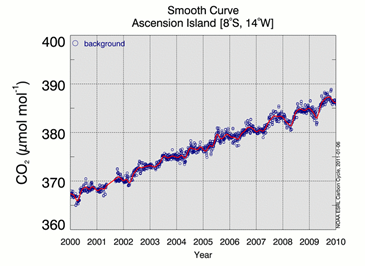
\includegraphics[keepaspectratio]{images/co2_Ascension.png}}

}

\caption{Figure 4: CO\(_2\) data from Ascension Island}

\end{figure}%

Solution

Critically, we have time series data, there are gaps, so a smooth curve
is fitted, using a quadratic as in the equation. However there is also a
need to include some cyclical terms, again introduced in the linear
modelling framework using sin and cosine terms. Very standard regression
modelling, but could and should also pick up on the fact there is no
mention of the error terms or assumptions and since this is time series,
we could expect that observations at a weekly scale are correlated, and
what effect that might have on the estimates and any inference --
i.e.~less independent data so we might expect the standard estimates of
our parameters to increase. An alternative approach may be to use a more
flexible method (e.g.~smoothing/GAM) to incorporate the seasonal pattern
but with a linear term for trend. Models could be compared using an
approximate F test. The advantage of the parametric approach adopted is
the (relative) ease of interpretation.

\end{tcolorbox}

\begin{tcolorbox}[enhanced jigsaw, colframe=quarto-callout-warning-color-frame, toptitle=1mm, toprule=.15mm, bottomtitle=1mm, titlerule=0mm, coltitle=black, left=2mm, rightrule=.15mm, arc=.35mm, colback=white, title={Task 4}, breakable, opacitybacktitle=0.6, opacityback=0, bottomrule=.15mm, leftrule=.75mm, colbacktitle=quarto-callout-warning-color!10!white]

A researcher monitors monthly water temperature (°C) at a river station
over 8 years (\(n=96\) observations, \(t = 1,\ldots,96\)). Water
temperature in rivers is well known to follow an annual seasonal cycle
driven by air temperature and solar radiation. Thus, the research fits
the harmonic regression model to the river temperature data:

\[
\mathbb{E}(Y_t) = \beta_0 + \beta_1\cos\left(\frac{2\pi t}{P}\right) + \beta_2\sin\left(\frac{2\pi t}{P}\right)
\] with the following R output:

\begin{verbatim}
lm(formula = temp ~ cos(2 * pi * t/P) + sin(2 * pi * t/P))

Coefficients:
                     Estimate Std. Error t value Pr(>|t|)    
(Intercept)           12.430      0.187   66.47   <2e-16 ***
cos(2 * pi * t/P)    -4.216      0.264  -15.97   <2e-16 ***
sin(2 * pi * t/P)     2.850      0.264   10.79   <2e-16 ***
---
Residual standard error: 1.826 on 93 degrees of freedom
Multiple R-squared:  0.834, Adjusted R-squared:  0.830 
F-statistic: 233.6 on 2 and 93 DF,  p-value: < 2.2e-16
\end{verbatim}

Answer the following:

\begin{enumerate}
\def\labelenumi{\arabic{enumi}.}
\tightlist
\item
  What value of \texttt{P} (i.e., the period) was used in this model?
\item
  State the fitted regression equation
\item
  Calculate the amplitude of the seasonal cycle.
\end{enumerate}

Solution

\begin{enumerate}
\def\labelenumi{\arabic{enumi}.}
\tightlist
\item
  P = 12 months --- data is monthly and one full annual cycle spans 12
  observations.
\item
  \(\widehat{\text{temp}}_t = 12.430 - 4.216\cos(2\pi t/12) + 2.850\sin(2\pi t/12)\)
\item
  \(\sqrt{(-4.216)^2+2.85^2} \approx 5.09.\)
\end{enumerate}

\end{tcolorbox}

\begin{tcolorbox}[enhanced jigsaw, colframe=quarto-callout-warning-color-frame, toptitle=1mm, toprule=.15mm, bottomtitle=1mm, titlerule=0mm, coltitle=black, left=2mm, rightrule=.15mm, arc=.35mm, colback=white, title={Task 5}, breakable, opacitybacktitle=0.6, opacityback=0, bottomrule=.15mm, leftrule=.75mm, colbacktitle=quarto-callout-warning-color!10!white]

The following excerpt is taken from the European Environment Agency web
site, concerning one of their key indicators (CSI012) for European
temperature (accessed Jan 2010):

\emph{``The Earth has experienced considerable temperature increases in
the last 100 years, especially in the most recent decades. These changes
are unusual in terms of both magnitude and rate of change. The rate of
change in the global average temperature is accelerating from
0.08}\(^\circ\)C per decade over the last 100 years, to 0.13\(^\circ\)C
per decade over the past 50 years up to 0.23\(^\circ\)C per decade over
the last 10 years (all values represent land \& ocean area) (IPCC,
2007a). As such the indicative target (to keep climate change within
`safe' limits) of 0.2\(^\circ\)C per decade has been exceeded in the
recent years.''

The figure below shows the time series plot of the CSI012 indicator,
which has been developed to address specific policy issues concerning
the trend and rate of change in the European annual and seasonal
temperature.

\begin{figure}[H]

{\centering 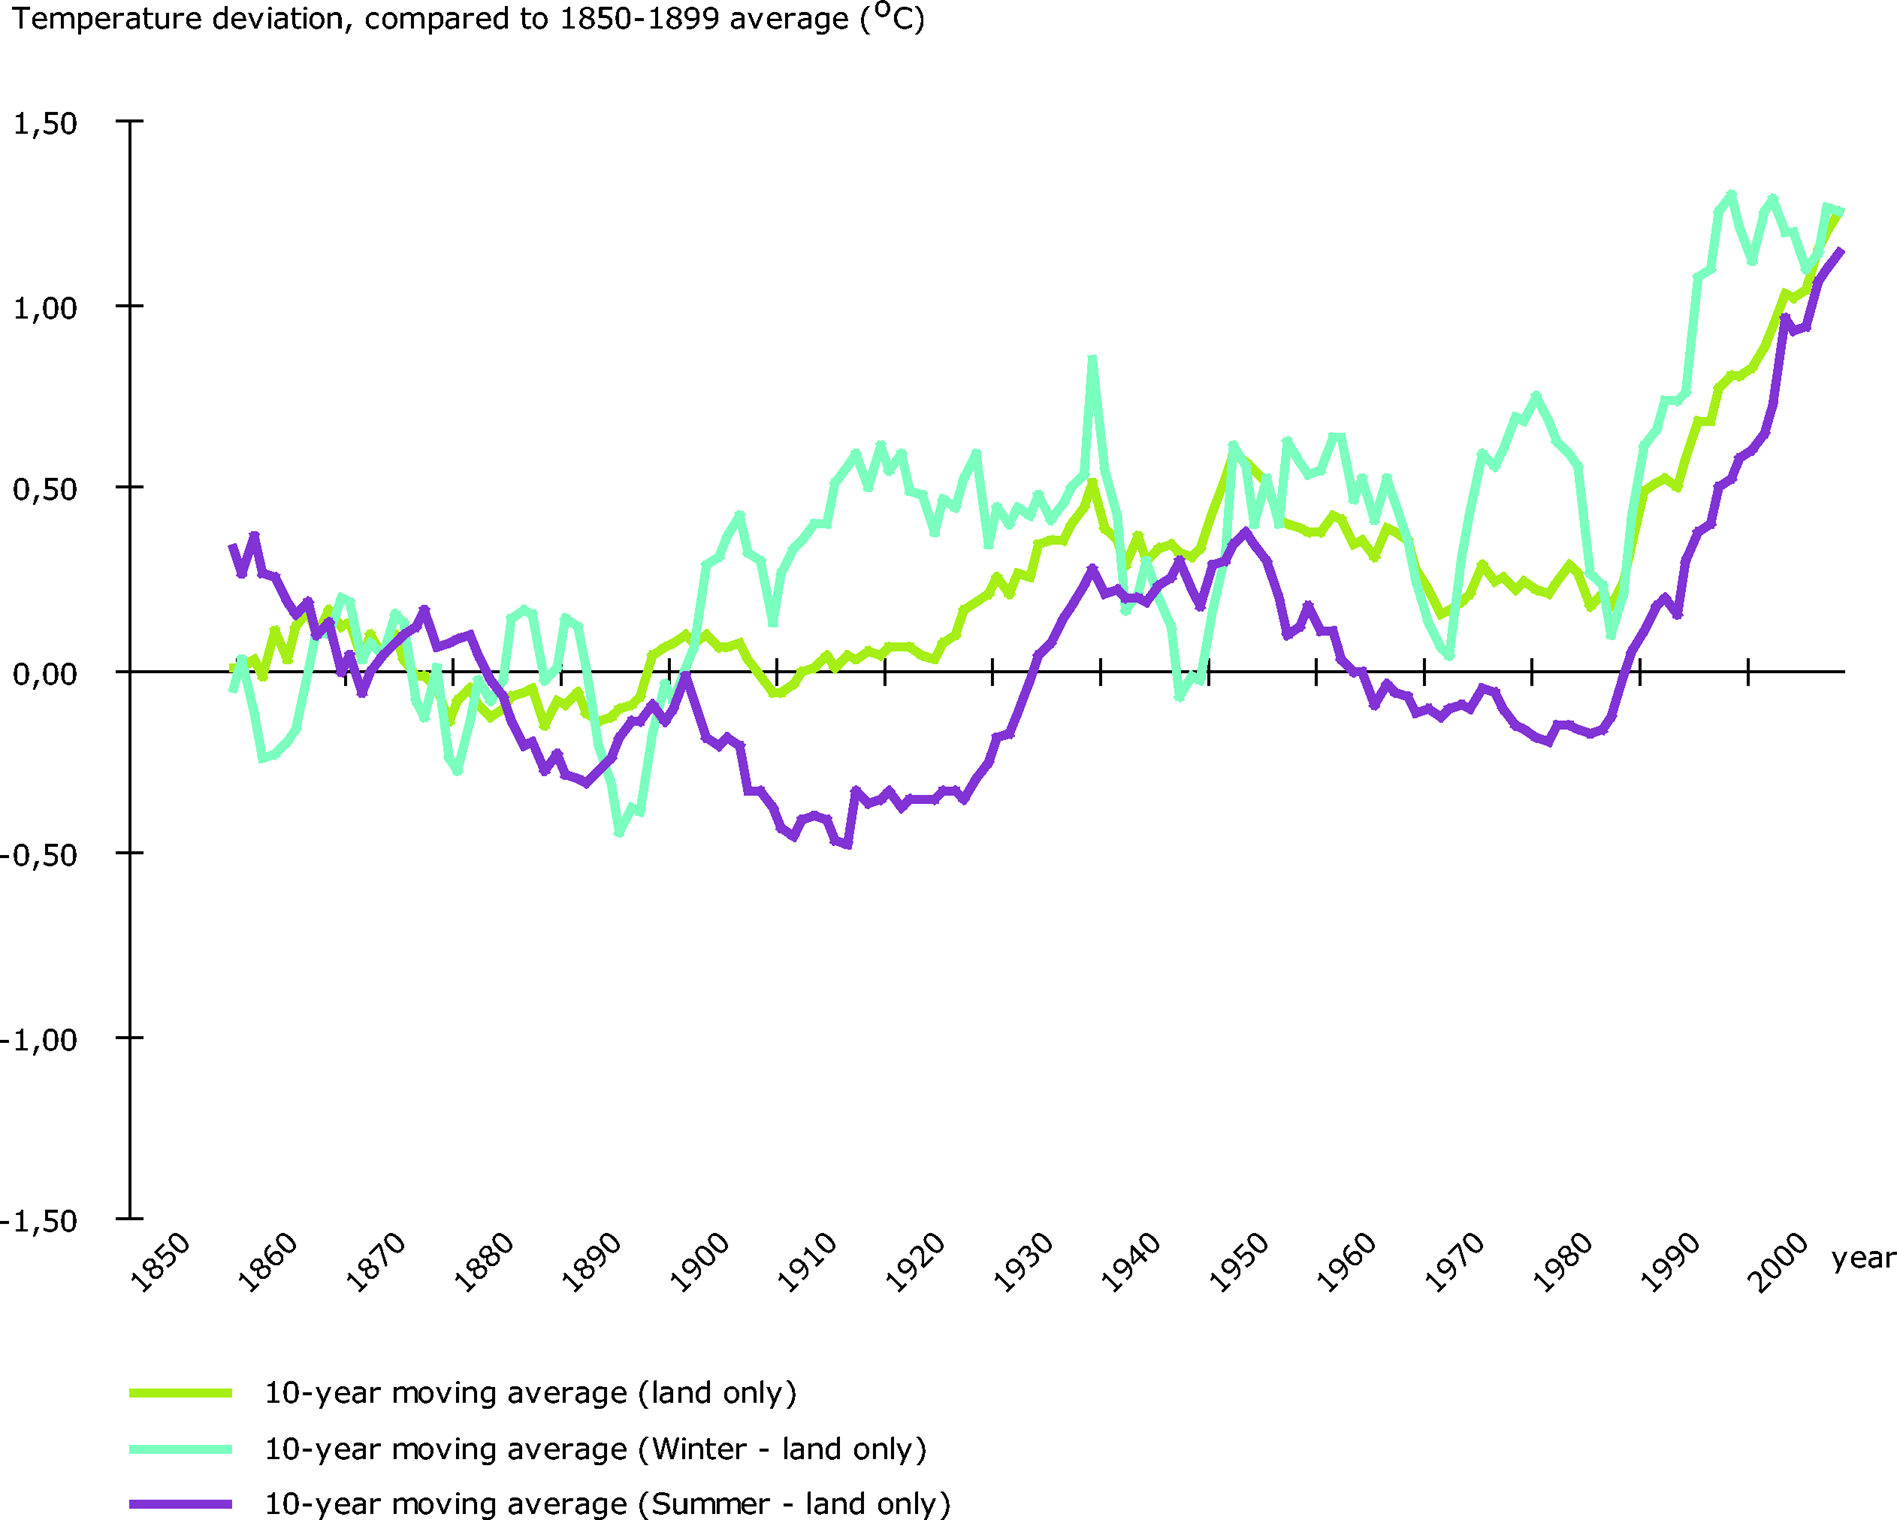
\includegraphics[width=6.44792in,height=\textheight,keepaspectratio]{images/csi012.png}

}

\caption{Figure 5: CSI012 European Land Temperature Deviations}

\end{figure}%

Discuss critically the statement and the above figure and how they might
be related. Suggest how you might model such temperature data above to
address the policy issues.

Solution

This example is again all about trends, expressed one presumes as a
linear trend, and a slope in the quote. The interesting thing is that
the slope is different in different time periods and over different
lengths of time. Again, no uncertainty is quoted. The plot shows
deviations using a 10 year moving average, so a smoothed plot, and we
can also see differences between summer and winter, suggesting
temperature change may indeed be occurring at different rates in
different times of the year. How might we model absolute temperature and
the deviations? We can certainly imagine therefore that temperature will
have a strong seasonal cycle (so could use a harmonic regression), that
a simple linear regression is not likely to be complex enough since the
rate of change is changing, so could fit some sort of piecewise
regression but what is the justification for the changepoints? Or we
could fit some sort of smooth curve (not necessarily monotonic).

\end{tcolorbox}

\begin{tcolorbox}[enhanced jigsaw, colframe=quarto-callout-warning-color-frame, toptitle=1mm, toprule=.15mm, bottomtitle=1mm, titlerule=0mm, coltitle=black, left=2mm, rightrule=.15mm, arc=.35mm, colback=white, title={Task 6}, breakable, opacitybacktitle=0.6, opacityback=0, bottomrule=.15mm, leftrule=.75mm, colbacktitle=quarto-callout-warning-color!10!white]

Suppose the following change point detection model of the form

\[Y_i = \alpha_1 + \beta_1x_i - (\beta_1-\beta_2)(x_i-c)_+ + \varepsilon_i\]
where
\((x - c)_+ = \begin{cases} 0 & \text{if } \ x < c\\ x- c & \text{if } x \geq c \end{cases}\)

Show that

\begin{enumerate}
\def\labelenumi{\arabic{enumi}.}
\tightlist
\item
  When \(x_i < c\), \(\mathbb{E}(Y_i) = \alpha_1 + \beta_1x_i\)
\item
  When \(x_i \geq c\), \(\mathbb{E}(Y_i) =  \alpha_2 + \beta_2 x_i\)
  such that \(\alpha_2 = \alpha_1 + (\beta_1 - \beta_2)c\)
\end{enumerate}

Solution

\begin{enumerate}
\def\labelenumi{\arabic{enumi}.}
\tightlist
\item
  when \(x_i < c\),
  \(\mathbb{E}(Y_i) = \alpha_1 + \beta_1x_i - (\beta_1-\beta_2)\overbrace{(x_i-c)_+}^{0}  = \alpha_1 + \beta_1 x_i\)
\item
  When \(x_i \geq c\),
\end{enumerate}

\[
\begin{align}
\mathbb{E}(Y_i) &=\alpha_1 + \beta_1x_i - (\beta_1-\beta_2)(x_i-c)\\
&=\alpha_1 + \beta_1x_i - \beta_1x_i+ \beta_1 c +\beta_2 x_i - \beta_2 c\\
&=\alpha_1 + \beta_1 c  - \beta_2 c + \beta_2 x_i \\
&=\alpha_1 + c (\beta_1   - \beta_2) + \beta_2 x_i  \quad \color{grey}{\text{setting } \alpha_2 = \alpha_1 + c (\beta_1   - \beta_2)} \\
&= \alpha_2 + \beta_2 x_i
\end{align}
\]

\end{tcolorbox}

\begin{tcolorbox}[enhanced jigsaw, colframe=quarto-callout-warning-color-frame, toptitle=1mm, toprule=.15mm, bottomtitle=1mm, titlerule=0mm, coltitle=black, left=2mm, rightrule=.15mm, arc=.35mm, colback=white, title={Task 7}, breakable, opacitybacktitle=0.6, opacityback=0, bottomrule=.15mm, leftrule=.75mm, colbacktitle=quarto-callout-warning-color!10!white]

The figure below shows a regression example from a paper in Science
(Johnson et al, 2014) which investigated the rate of thinning of the
Pine Island glacier. They fit a \textbf{2-segment, piecewise-linear
age-elevation history to the Mt Moses dat}.

\begin{center}
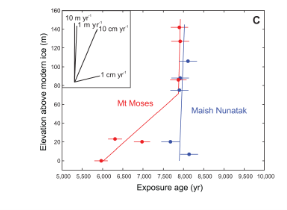
\includegraphics[width=3.98958in,height=\textheight,keepaspectratio]{images/MtMoses.png}
\end{center}

Explain what the phrase in bold above means, and write down the equation
for a 2 stage regression, assuming a \textbf{known changepoint}. Explain
how the parameters of the model can be estimated. Comment briefly on the
figure above.

Solution

The model that the authors have fitted is one where there are two
straight lines which are constrained to meet at a changepoint.

A change-point could be defined as a point that separates a series of
observations into two groups, each following a different model, in this
case a different slope and intercept.

Known changepoint:

\[f(x_i) = \begin{cases} \alpha_1 + \beta_1x_i \hspace{1cm} x_i\leq \delta\\ \alpha_2 + \beta_2 x_i \hspace{1cm} \delta \leq x_i \end{cases}\]

constrained such that

\[\alpha_1 + \beta_1 \delta = \alpha_2 + \beta_2 \delta\]

Parameters can then be estimated by ordinary least squares. Plot shows
the diverging line, no uncertainty estimates, nor justification of where
the changepoint occurs.

\end{tcolorbox}

\section{Part B: Models for extremes}\label{part-b-models-for-extremes}

\begin{tcolorbox}[enhanced jigsaw, colframe=quarto-callout-warning-color-frame, toptitle=1mm, toprule=.15mm, bottomtitle=1mm, titlerule=0mm, coltitle=black, left=2mm, rightrule=.15mm, arc=.35mm, colback=white, title={Task 8}, breakable, opacitybacktitle=0.6, opacityback=0, bottomrule=.15mm, leftrule=.75mm, colbacktitle=quarto-callout-warning-color!10!white]

If \(X_1, \dots, X_n\) is a sequence of independent standard exponential
\(Exp(1)\) variables,

\begin{enumerate}
\def\labelenumi{(\alph{enumi})}
\tightlist
\item
  Show that \(F(x)= 1-e^{-x}\) for \(x> 0\).
\item
  Show that, for \(a_n=1\) and \(b_n=\log(n)\), the limit distribution
  of \(M_n\) as \(n \rightarrow \infty\) is the Gumbel distribution,
  corresponding to \(\zeta = 0\) in the GEV family.
\end{enumerate}

Solution

\begin{enumerate}
\def\labelenumi{(\alph{enumi})}
\item
  If \(X_1, \dots, X_n \sim Exp(1)\),

  \begin{itemize}
  \tightlist
  \item
    range of \(x\) is \(X>0\)
  \item
    pdf of \(Exp(\lambda)\) is \(f(x) = \lambda e^{-\lambda x}\), so for
    \(Exp(1)\), \(f(x) = e^{-x}\)
  \end{itemize}
\end{enumerate}

\[\begin{split}\therefore F(x) &= P(X \leq x)\\ &= \int_0^x f(t) dt\\ &= [-e^{-t}]_0^x\\ &= -e^{-x} - (-e^0)\\ &= 1 - e^{-x} \hspace{1cm} (\text{for } x>0)\end{split}\]

\begin{enumerate}
\def\labelenumi{(\alph{enumi})}
\setcounter{enumi}{1}
\tightlist
\item
  Let \(M_n = \max\{X_1, \dots, X_n\}\), let \(a_n = 1\) and let
  \(b_n = \log(n)\). Then:
\end{enumerate}

\[Pr\left\{\frac{M_n - b_n}{a_n} \leq z \right\} = F^n(a_nz + b_n) \rightarrow G(z) \text{ as } n \rightarrow \infty\]
\[\begin{split} F_n(a_nz + b_n) & = F^n(z+\log(n))\\ & = [1 - e^{-(z+\log(n))}]^n\\ &\rightarrow \left[1-\frac{e^{-z}}{n} \right]^n \ \text{ as } n \rightarrow \infty\\ &= -\exp(-\exp(-z))\end{split}\]

{\marginnote{\begin{footnotesize}Note:
\[\exp(x) = \lim_{n \rightarrow \infty}\left( 1+\frac{x}{n}\right)^n \ \ \ \ \ \ \ \ \]\end{footnotesize}}}

\end{tcolorbox}

\begin{tcolorbox}[enhanced jigsaw, colframe=quarto-callout-warning-color-frame, toptitle=1mm, toprule=.15mm, bottomtitle=1mm, titlerule=0mm, coltitle=black, left=2mm, rightrule=.15mm, arc=.35mm, colback=white, title={Task 9}, breakable, opacitybacktitle=0.6, opacityback=0, bottomrule=.15mm, leftrule=.75mm, colbacktitle=quarto-callout-warning-color!10!white]

If \(X_1, \dots, X_n\) is a sequence of independent standard exponential
\(Exp(\lambda)\) variables,

\begin{enumerate}
\def\labelenumi{(\alph{enumi})}
\tightlist
\item
  Show that \(F_n(x)= (1-e^{-\lambda x})^n\) for \(x> 0\), where
  \(F_n(x)\) is the distribution of \(X(n)\).
\item
  Find the distribution function of \(X_{(1)}\), and show that
  \(X_{(1)}\) has an Exponential distribution with parameter
  \(n\lambda\).
\end{enumerate}

Solution

\begin{enumerate}
\def\labelenumi{(\alph{enumi})}
\tightlist
\item
  \(F(x) = 1 - e^{-\lambda x}\)
\end{enumerate}

\[\begin{split} F_n(x) &= [P(X \leq x)]^n\\ &=\left[ \int_0^x f(t) dt\right]^n\\ &=\left[\int_0^x \lambda e^{-\lambda t} dt \right]^n\\ &=\left[ \left[ e^{-\lambda t}\right]_0^x\right]^n\\ &=\left[ 1 - e^{-\lambda x}\right]^n \end{split}\]

\begin{enumerate}
\def\labelenumi{(\alph{enumi})}
\setcounter{enumi}{1}
\tightlist
\item
  Let \(X_{(1)} = \min\left\{X_1, \dots, X_n \right\}\). Then:
\end{enumerate}

\[\begin{split} \Pr\left\{ X_{(1)} \leq t\right\} &= \Pr\left\{ \min\left\{X_1, \dots, X_n \right\} \leq t\right\}\\ &= 1 - \Pr\left\{ \min\left\{X_1, \dots, X_n \right\} \geq t\right\}\\ &= 1 - \Pr \left\{ X_i \geq t \ \text{for all} \ i\right\}\\ &= 1 - (e^{-\lambda t})^n\\ &= 1 - e^{-\lambda nt} \end{split}\]
\[\therefore X_{(1)} \sim Exp(n \lambda)\]

\end{tcolorbox}

\begin{tcolorbox}[enhanced jigsaw, colframe=quarto-callout-warning-color-frame, toptitle=1mm, toprule=.15mm, bottomtitle=1mm, titlerule=0mm, coltitle=black, left=2mm, rightrule=.15mm, arc=.35mm, colback=white, title={Task 10}, breakable, opacitybacktitle=0.6, opacityback=0, bottomrule=.15mm, leftrule=.75mm, colbacktitle=quarto-callout-warning-color!10!white]

\begin{enumerate}
\def\labelenumi{(\alph{enumi})}
\tightlist
\item
  Daily wind speed data are available for a location in the Netherlands.
  A POT modelling approach has been used to model the data. The figure
  below shows a mean residual life plot for the series. Comment on how
  you could use this plot to identify a suitable threshold for the POT
  model. What threshold would you select here?
\end{enumerate}

\begin{center}
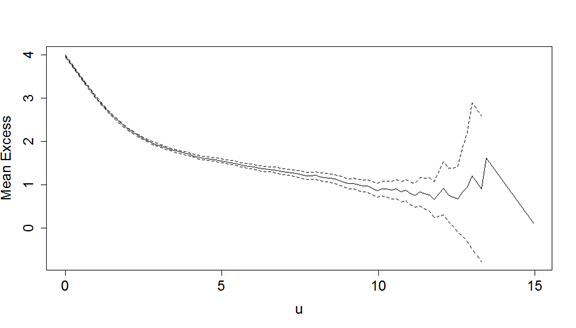
\includegraphics[width=5.16667in,height=\textheight,keepaspectratio]{images/windspeed_Netherlands.png}
\end{center}

\begin{enumerate}
\def\labelenumi{(\alph{enumi})}
\setcounter{enumi}{1}
\tightlist
\item
  The figure below shows the diagnostic plots for a fitted POT model for
  the wind speed data. Comment on the model fit using these plots.
\end{enumerate}

\begin{center}
\pandocbounded{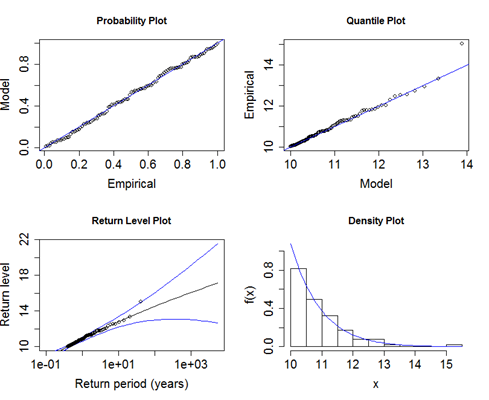
\includegraphics[keepaspectratio]{images/windspeed_Netherlands_model.png}}
\end{center}

\begin{enumerate}
\def\labelenumi{(\alph{enumi})}
\setcounter{enumi}{2}
\tightlist
\item
  The threshold selected was 10. Comment on this choice using the
  sensitivity analysis below.
\end{enumerate}

\begin{center}
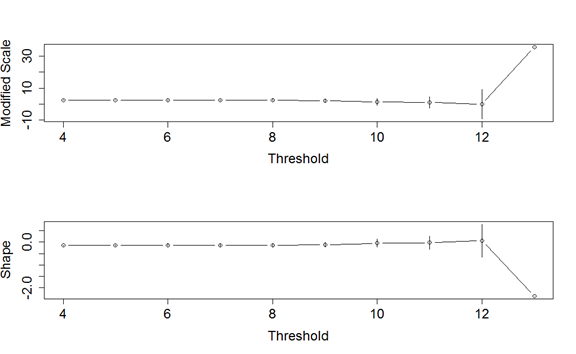
\includegraphics[width=5.03125in,height=\textheight,keepaspectratio]{images/windspeed_Netherlands_sens.png}
\end{center}

\begin{enumerate}
\def\labelenumi{(\alph{enumi})}
\setcounter{enumi}{3}
\tightlist
\item
  The R output for the model is shown below.
\end{enumerate}

\begin{verbatim}
$threshold
[1] 10

$nexc
[1] 105

$conv
[1] 0

$nllh
[1] 92.17218

$mle
[1]  0.9278907 -0.0473220

$rate
[1] 0.00684485

$se
[1] 0.12364549 0.09084164
\end{verbatim}

Estimate the 1 in 100 year wind speed.

Solution

\begin{enumerate}
\def\labelenumi{(\alph{enumi})}
\item
  Looking for area where (after taking confidence bands into account)
  the mean excess is linearly related to the threshold. Not immediately
  obvious, somewhat subjective. I would say somewhere between 10 and 13.
  Start as low as possible so 10 would be a good threshold to start
  with.
\item
  Quantile and probability plots both have good agreement between points
  (corresponding to the sample) and the theoretical line, therefore the
  fit seems reasonable. Histogram also seems to have good agreement
  between the sample and the solid line which represents the estimated
  density using the fitted model. Have to be careful when interpreting
  histograms as interpretation can change with the number of bins used,
  particularly when the sample size is small. Return level plot, points
  lie within confidence interval in general. Another indication the
  model is suitable.
\item
  The threshold value of 10 seems like a good threshold. There is very
  little variability in the sensitivity analysis fit, the parameter
  estimates seem constant across a range of thresholds, only at 12 and
  above do estimates seem to vary. Maybe could argue we could look at
  thresholds even lower than 10 ---- need to balance what is truly
  extreme, while ensuring there is sufficient data available above the
  threshold to use to estimate our model.
\end{enumerate}

\end{tcolorbox}

\begin{tcolorbox}[enhanced jigsaw, colframe=quarto-callout-warning-color-frame, toptitle=1mm, toprule=.15mm, bottomtitle=1mm, titlerule=0mm, coltitle=black, left=2mm, rightrule=.15mm, arc=.35mm, colback=white, title={Task 11}, breakable, opacitybacktitle=0.6, opacityback=0, bottomrule=.15mm, leftrule=.75mm, colbacktitle=quarto-callout-warning-color!10!white]

The generalized extreme value distribution (GEV) has three parameters
and distribution function

\[G(z) = \exp \left\{ -\left[ 1+\xi\frac{(z_i - \mu)}{\sigma}\right]^{\frac{-1}{\xi}}\right\}\]

GEV is often used when modelling block maxima. Identify the particular
family and write down its distribution function when \(\xi\) is assumed
equal to 0.

Show that when \(G(z_p) =1-p\), then

\[z_p = \begin{cases} \mu - \sigma \frac{[1-\{-\log(1-p)\}^{-\xi}]}{\xi} & \text{for } \xi \neq 0\\ 
\mu - \sigma[\log\{-\log(1-p)\}] & \text{for } \xi = 0\end{cases}\]

For the distribution \(G\) in the case \(\xi=0\), show that if \(z_p\)
is plotted against \(\log[–\log(1-p)]\), the plot should be linear.

Solution

\[G(z) = \exp \left\{ -\left[ 1+\xi\frac{(z - \mu)}{\sigma}\right]^{\frac{-1}{\xi}}\right\}\]

Set \(G(z_p) = 1 - p\) and solve equation above for \(z_p\):

\[\begin{split} \exp \left\{ -\left[ 1+\xi\frac{(z_p - \mu)}{\sigma}\right]^{\frac{-1}{\xi}}\right\} &= 1 - p\\
\left\{ -\left[ 1+\xi\frac{(z_p - \mu)}{\sigma}\right]^{\frac{-1}{\xi}}\right\} &= \log(1-p)\\
-\left[ 1+\xi\frac{(z_p - \mu)}{\sigma}\right] &= \log(1-p)^{-\xi}\\
\left[ 1+\xi\frac{(z_p - \mu)}{\sigma}\right] &= -\log(1-p)^{-\xi}\\
\xi\frac{(z_p - \mu)}{\sigma} &= \{ -\log(1-p)^{-\xi}\}-1\\
\frac{(\mu - z_p)}{\sigma} &= \frac{1}{\xi}[1-(-\log(1-p)^{-\xi})]\\
-z_p &= -\mu + \frac{\sigma}{\xi}(1-(-\log(1-p)^{-\xi}))\\z_p &= \mu - \frac{\sigma}{\xi}(1-(-\log(1-p)^{-\xi}))\end{split}\]

When \(\xi = 0\), we have a Gumbel distribution:

\[\begin{split}\exp\left[ -\exp\left( \frac{-(z_p - \mu)}{\sigma}\right)\right] &= 1-p\\
\left[ -\exp\left( \frac{-(z_p - \mu)}{\sigma}\right)\right] &=\log(1-p)\\
\left( \frac{-(z_p - \mu)}{\sigma}\right) &= \log(-\log(1-p))\\
-z_p + \mu &= \sigma\log(-\log(1-p))\\
-z_p &= -\mu + \sigma\log(-\log(1-p))\\
z_p &= \mu - \sigma\log(-\log(1-p))\end{split}\]

\(z_p\) is the return level associated with the return period \(1/p\).

Let \(s_p = \log(-\log(1-p))\). Then
\(z_p = \mu - \sigma\log(-\log(1-p)) = \mu - \sigma s_p\) when
\(\xi = 0\). Therefore, \(z_p\) is linearly related to
\(\log(-\log(1-p))\) in the case \(\xi = 0\).

\end{tcolorbox}




\end{document}
